\documentclass[10pt]{article}

\usepackage[a4paper,margin=0.75in]{geometry}
\usepackage[T1]{fontenc}
\usepackage[utf8]{inputenc}
\usepackage{times}
\usepackage{graphicx}
\usepackage{xcolor}
\usepackage{amsmath}
\usepackage{booktabs}
\usepackage{url}
\usepackage{hyperref}
\usepackage{caption}
\usepackage{placeins}
\usepackage{tikz}
\usetikzlibrary{arrows.meta,positioning,fit,calc,backgrounds}
\pgfdeclarelayer{background}
\pgfsetlayers{background,main}

\hypersetup{
    colorlinks=true,
    linkcolor=black,
    citecolor=black,
    urlcolor=blue!60!black
}

\setlength{\parskip}{0.35em}
\setlength{\parindent}{1em}
\captionsetup{font=small,labelfont=bf}
\sloppy

\title{\textbf{L4S-Aware Queueing in BMv2: ECN-Based Class Separation and Dynamic Threshold Control}}
\author{
Sooraj Subramanian M. S. (CS25S031) \and
Sk Fardeen Hossain (CS25S010) \and
Kunal Umaji (CS25S020)
}
\date{CS6045 Software Defined Networks --- Course Project Report}

\begin{document}
\maketitle

\noindent\textbf{Repository link:} TODO: insert public GitHub URL.

\begin{abstract}
Low-Latency, Low-Loss, and Scalable Throughput (L4S) separates scalable ECN-capable traffic from conventional Classic traffic so that shallow congestion marking can be applied to latency-sensitive flows without forcing all traffic into the same queueing behavior. This project implements an L4S-aware queueing prototype on BMv2 using P4 and Mininet. The P4 dataplane parses the IPv4 ECN field, classifies ECT(1) and CE packets as L4S, classifies Not-ECT and ECT(0) packets as Classic, maps the two classes to separate BMv2 priority queues, applies class-specific ECN marking in egress using queue-depth thresholds, and exports queue telemetry through registers. A lightweight Python controller reads these registers through \texttt{simple\_switch\_CLI} and dynamically adjusts the L4S marking threshold and Classic protection parameters.

The prototype is a target-constrained approximation rather than a standards-complete implementation of DualQ Coupled AQM. BMv2 exposes priority queues and queue metadata, but it does not allow the P4 program to implement an arbitrary coupled traffic scheduler. The project therefore focuses on a concrete SDN question: whether runtime queue telemetry and control-plane threshold updates can reduce the Classic-throughput penalty created by L4S-favoring priority service. The evaluation compares a static two-queue configuration against a dynamic-threshold configuration under mixed L4S and Classic TCP traffic on a 10 Mbps bottleneck. With static thresholds, L4S obtains 7.82 Mbps and Classic obtains 1.71 Mbps, producing a Jain fairness index of 0.709. Across a 6 by 6 dynamic-controller step-size sweep, L4S throughput lies between 3.61 and 4.25 Mbps, Classic throughput lies between 5.00 and 5.64 Mbps, and Jain fairness lies between 0.953 and 0.990. The results show that dynamic thresholding and Classic protection substantially improve coexistence, but the improvement is obtained by reducing L4S throughput share. The main outcome is a reproducible BMv2/P4 testbed and an empirical characterization of the fairness tradeoff in this L4S-aware approximation.
\end{abstract}

\section{Introduction}

L4S is motivated by the observation that conventional queueing and congestion-control interactions can create persistent queue buildup at bottlenecks. ECN-based marking provides a way for the network to signal congestion before packet loss occurs, and scalable congestion controls such as DCTCP can react to frequent shallow marking more smoothly than conventional TCP. In the L4S architecture, ECT(1) is used to identify scalable low-latency traffic, while Not-ECT and ECT(0) remain associated with the Classic service class. A dual-queue design can then apply different marking and scheduling behavior to the two classes.

A naive implementation of this idea is not sufficient. If L4S packets are simply placed in a strict higher-priority queue, the L4S class can dominate the bottleneck whenever both classes are backlogged. Classic traffic then receives only residual service, even though coexistence is a central design requirement of L4S. Conversely, if Classic traffic is protected too aggressively, the intended L4S benefit may be weakened. The practical problem is therefore a control problem at the bottleneck: the system must expose enough preference for L4S traffic to maintain class separation, while preventing Classic traffic from being pushed into starvation-like behavior.

This project investigates that problem in the BMv2 software switch. BMv2 is suitable for an SDN course project because it supports P4\_16, exposes queue metadata in the v1model architecture, and supports multiple priority queues. At the same time, BMv2 imposes an important limitation: the traffic manager is not itself fully programmable from P4. The dataplane can classify packets, set queue priority, read queue metadata in egress, update registers, and modify headers, but it cannot directly implement a full DualQ Coupled AQM scheduler. The implemented system is therefore designed as a measurable approximation using the mechanisms BMv2 actually provides.

The project makes three contributions. First, it implements a P4 dataplane that performs ECN-based class separation, queue selection, egress ECN marking, queue telemetry export, and basic IPv4 forwarding inside BMv2. Second, it implements a control-plane feedback loop that polls queue-state registers and adjusts L4S and Classic threshold parameters at runtime. Third, it provides an end-to-end Mininet evaluation harness using DCTCP-based L4S traffic, Cubic-based Classic traffic, packet capture, \texttt{iperf3} measurements, confidence-interval computation, and controller-step ablation plots.

\section{Background and Design Constraints}

The IPv4 ECN field contains two bits. Not-ECT identifies packets that are not ECN-capable; ECT(0) and ECT(1) identify ECN-capable packets; CE identifies packets that have already been congestion-marked. In the L4S interpretation used here, ECT(1) and CE belong to the L4S class, while Not-ECT and ECT(0) belong to the Classic class. This classification follows the core L4S convention and gives the switch a simple per-packet rule that can be implemented directly in the P4 ingress pipeline.

The congestion-control behavior of the senders matters because ECN marking is only useful if end hosts react to it. The L4S sender uses DCTCP, which responds to the fraction of marked packets. Since Linux DCTCP normally emits ECT(0), the traffic script rewrites the ECN field of outgoing TCP packets to ECT(1) using an \texttt{iptables} mangle rule. The Classic sender uses TCP Cubic and can be run with ECN enabled, producing ECT(0) traffic that is still classified into the Classic queue. This setup is not a production L4S stack, but it is sufficient for a controlled experiment in which the switch can distinguish the two traffic classes.

BMv2 provides the target features needed for the prototype. The ingress pipeline can write \texttt{standard\_metadata.priority}, allowing packets to be assigned to one of two priority queues when \texttt{simple\_switch} is launched with two priority queues. The egress pipeline can read queue metadata such as \texttt{deq\_qdepth}, \texttt{enq\_qdepth}, and \texttt{deq\_timedelta}. The P4 program can also read and write registers that are visible to the control plane through the BMv2 CLI. These mechanisms define the feasible design: class separation is performed in ingress, marking and telemetry export are performed in egress, and threshold adaptation is performed by a controller outside the dataplane.

The main design constraint is that this is not a programmable traffic-manager target. The implementation cannot replace BMv2's scheduler with a standards-faithful DualQ Coupled AQM scheduler. It can only approximate L4S-aware behavior using priority queues, CE marking, register-based telemetry, and controller updates. The report therefore evaluates the prototype as a BMv2 approximation and does not claim RFC-level conformance.

\section{System Architecture and Implementation}

Figure~\ref{fig:system-architecture} shows the implemented architecture. Four senders transmit through a single BMv2 switch toward one receiver. Hosts \texttt{h1} and \texttt{h2} generate L4S traffic, hosts \texttt{h3} and \texttt{h4} generate Classic traffic, and host \texttt{h5} receives both classes. The switch acts as the bottleneck and runs the P4 dataplane. Ingress classifies packets by ECN codepoint and selects the appropriate priority queue, while egress performs CE marking and exports queue telemetry. A Python controller runs outside the dataplane, polls the telemetry registers, and updates the threshold and protection parameters used by the switch.

% Figure 1 is a TikZ figure stored inside report/figures/.
% Since this main TeX file is intended to live in report/, the relative path below is correct.
\begin{figure}[t]
\centering
\resizebox{\linewidth}{!}{%
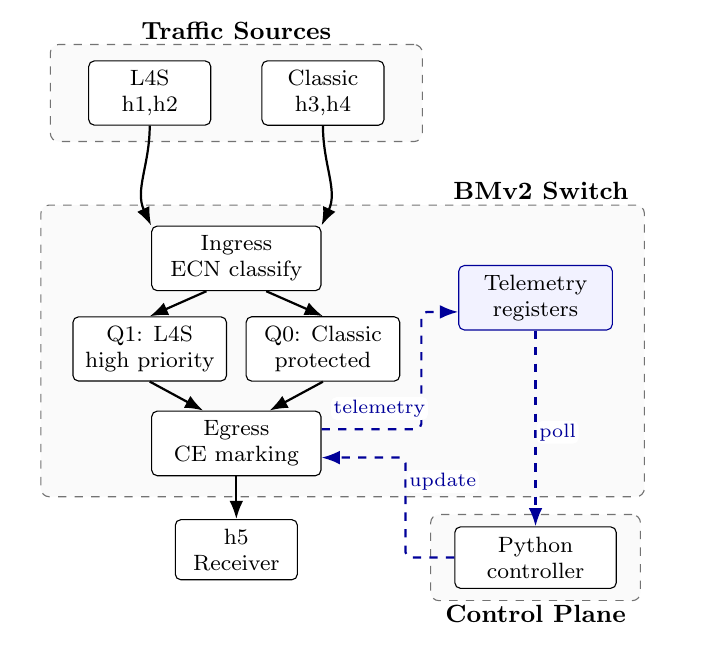
\begin{tikzpicture}[
    font=\footnotesize,
    >=Latex,
    data/.style={->, thick, rounded corners=2pt},
    ctrl/.style={->, thick, dashed, draw=blue!60!black, rounded corners=2pt},
    box/.style={
        draw=black,
        rounded corners=2pt,
        align=center,
        minimum width=2.15cm,
        minimum height=0.82cm,
        fill=white
    },
    smallbox/.style={
        draw=black,
        rounded corners=2pt,
        align=center,
        minimum width=1.55cm,
        minimum height=0.72cm,
        fill=white
    },
    queue/.style={
        draw=black,
        rounded corners=2pt,
        align=center,
        minimum width=1.95cm,
        minimum height=0.78cm,
        fill=white
    },
    regbox/.style={
        draw=blue!60!black,
        rounded corners=2pt,
        align=center,
        minimum width=1.95cm,
        minimum height=0.72cm,
        fill=blue!5
    },
    group/.style={
        draw=black!55,
        dashed,
        rounded corners=3pt,
        fill=gray!4
    },
    grouptitle/.style={font=\small\bfseries, fill=white, inner sep=1.5pt}
]

% Stable crop.
\path[use as bounding box] (-2.65,-3.35) rectangle (5.55,4.38);

% --------------------------------------------------
% Traffic sources
% --------------------------------------------------
\node[smallbox] (l4s_src) at (-1.10,3.55) {L4S\\h1,h2};
\node[smallbox] (cl_src)  at ( 1.10,3.55) {Classic\\h3,h4};

% --------------------------------------------------
% BMv2 data path
% --------------------------------------------------
\node[box] (ingress) at (0.0,1.45) {Ingress\\ECN classify};

\node[queue] (q1) at (-1.10,0.30) {Q1: L4S\\high priority};
\node[queue] (q0) at ( 1.10,0.30) {Q0: Classic\\protected};

\node[box] (egress) at (0.0,-0.90) {Egress\\CE marking};
\node[smallbox] (rx) at (0.0,-2.25) {h5\\Receiver};

\node[regbox] (regs) at (3.80,0.95) {Telemetry\\registers};
\node[box, minimum width=2.05cm, minimum height=0.78cm] (ctrl) at (3.80,-2.35) {Python\\controller};

% Helper coordinates for separate control-arrow entry/exit points.
\coordinate (egtele) at ([yshift=0.18cm]egress.east);
\coordinate (egupdate) at ([yshift=-0.18cm]egress.east);
% Telemetry path is routed through the open gap to the right of Q0,
% avoiding overlap with the Q0 node before entering the register block.
\coordinate (telebus) at (2.35,-0.72);
\coordinate (regwrite) at ([yshift=-0.18cm]regs.west);
\coordinate (updatebus) at ($(ctrl.west)+(-0.62cm,0)$);

% --------------------------------------------------
% Background groups, fitted after nodes so the switch box clears egress.
% --------------------------------------------------
\begin{pgfonlayer}{background}
\node[group, fit=(l4s_src)(cl_src), inner xsep=0.48cm, inner ysep=0.20cm] (srcgroup) {};
\node[group, fit=(ingress)(q1)(q0)(egress)(regs), inner xsep=0.40cm, inner ysep=0.26cm] (swgroup) {};
\node[group, fit=(ctrl), inner xsep=0.30cm, inner ysep=0.15cm] (ctrlgroup) {};
\end{pgfonlayer}

\node[grouptitle] at ($(srcgroup.north)+(0,0.17)$) {Traffic Sources};
\node[grouptitle, anchor=east] at ($(swgroup.north east)+(-0.15,0.17)$) {BMv2 Switch};
\node[grouptitle] at ($(ctrlgroup.south)+(0,-0.16)$) {Control Plane};

% --------------------------------------------------
% Data-plane arrows: kept separate to avoid ambiguous split/merge arrows.
% --------------------------------------------------
\draw[data] (l4s_src.south) to[out=-90,in=115] (ingress.north west);
\draw[data] (cl_src.south)  to[out=-90,in=65]  (ingress.north east);

\draw[data] ([xshift=-0.38cm]ingress.south) -- (q1.north);
\draw[data] ([xshift= 0.38cm]ingress.south) -- (q0.north);

\draw[data] (q1.south) -- ([xshift=-0.42cm]egress.north);
\draw[data] (q0.south) -- ([xshift= 0.42cm]egress.north);

\draw[data] (egress.south) -- (rx.north);

% --------------------------------------------------
% Telemetry and control arrows.
% Egress writes telemetry into the register block from outside.
% The controller update arrow enters the egress block separately.
% --------------------------------------------------
\draw[ctrl] (egtele) --
    node[pos=0.58, above=3pt, fill=white, inner sep=1pt,
    text=blue!60!black] {\scriptsize telemetry}
    (telebus) -- (telebus |- regwrite) -- (regwrite);

\draw[ctrl] (regs.south) --
    node[pos=0.52, right, fill=white, inner sep=1pt,
    text=blue!60!black] {\scriptsize poll}
    (ctrl.north);

\draw[ctrl] (ctrl.west) -- (updatebus) |-
    node[pos=0.38, right, fill=white, inner sep=1pt,
    text=blue!60!black] {\scriptsize update}
    (egupdate);

\end{tikzpicture}%
}
\caption{System architecture of the L4S-aware BMv2 prototype. L4S and Classic traffic sources are classified using ECN at ingress, mapped to separate priority queues, and marked at egress. Queue telemetry is exported to registers, while the Python controller polls the telemetry and updates the egress marking policy.}
\label{fig:system-architecture}
\end{figure}


The P4 dataplane is divided into parser, ingress, egress, checksum, and deparser blocks. The parser extracts Ethernet and IPv4 headers. In ingress, the ECN field is inspected. ECT(1) and CE packets are assigned to the L4S class, while Not-ECT and ECT(0) packets are assigned to the Classic class. The selected class is written into local metadata and translated into \texttt{standard\_metadata.priority}, with L4S assigned to the higher-priority queue and Classic assigned to the lower-priority queue. The ingress pipeline also performs IPv4 forwarding using an LPM table and supports non-IPv4 forwarding through an L2 table, which is needed for ARP and basic Mininet connectivity.

Egress implements the marking and telemetry logic. The switch reads the current class threshold from a register, compares it with \texttt{standard\_metadata.deq\_qdepth}, and marks ECN-capable packets as CE when the threshold is exceeded. Not-ECT packets are not converted into CE. The egress pipeline also writes the latest queue depth, queue delay, enqueue-depth sample, and queue-growth estimate into registers. These exported values form the control-plane input used by the dynamic controller. Because the ECN field may be modified, the IPv4 checksum is recomputed before deparsing.

The static configuration alone is not enough to protect Classic traffic under overload. The dataplane therefore includes a small Classic-protection mechanism. Native Classic arrivals increment a bounded protection budget stored in a register. Later L4S arrivals can consume this budget and be demoted into the Classic queue. This mechanism is intentionally simple. It is not weighted fair queueing and it does not expose exact live Classic queue occupancy to ingress. Its purpose is to ensure that the presence of Classic demand can influence subsequent L4S queue assignment, even when strict priority would otherwise keep refilling the L4S queue.

The dynamic controller is implemented in Python. At each polling interval, it reads the L4S threshold, Classic threshold, Classic protection threshold, L4S queue depth, Classic queue depth, L4S delay, L4S growth, and Classic growth. It then applies a threshold policy with three actions: tighten, relax, or hold. The L4S threshold is tightened when Classic backlog is high, when L4S queue growth is high, or when L4S delay is high. The threshold is relaxed only when both queues are in a configured healthy region and neither queue is growing. When the decision reason is Classic backlog, the controller also increases Classic threshold and Classic protection settings. When queues are healthy, it relaxes those values toward lower bounds. Controller decisions are logged to a JSON-lines trace for debugging and reproducibility.

The topology script compiles the P4 program, launches \texttt{simple\_switch}, enables two priority queues, installs forwarding rules, initializes threshold registers, configures host routes and static ARP entries, disables offloads on Mininet interfaces, and starts either a static or dynamic experiment. The switch-to-receiver direction is rate-limited to create a visible bottleneck, and BMv2 queue depth/rate settings are configured so that egress queue metadata reflects the bottleneck behavior. The traffic scripts use \texttt{iperf3} to generate DCTCP-based L4S traffic and Cubic-based Classic traffic, while the receiver records \texttt{iperf3} JSON output and packet captures for post-processing.

\section{Experimental Methodology}

The final evaluation focuses on the behavior of the implemented dual-queue prototype under overload. Both L4S and Classic traffic are offered at 10 Mbps, while the bottleneck is configured at 10 Mbps. The sender links are configured at 100 Mbps, the nominal link delay is 5 ms, and the queue depth is 100 packets. Each run lasts 180 seconds. The reported throughput values are computed from receiver-side \texttt{iperf3} summaries.

Two configurations are compared. The static configuration uses fixed register values throughout the run, with an L4S threshold of 30 packets, a Classic threshold of 80 packets, and a Classic protection threshold of 16. This configuration represents a static two-queue L4S-aware design rather than a single FIFO baseline. The dynamic configuration uses the same dataplane but starts the controller. Its fairness-oriented profile initializes the L4S threshold at 8 packets, the Classic threshold at 100 packets, and the Classic protection threshold at 32. The controller then updates these values during the experiment. The dynamic ablation varies \texttt{relax\_step} and \texttt{tighten\_step} over $\{1,2,4,8,16,32\}$, producing a 6 by 6 grid. Each grid point is run for three trials, giving 108 dynamic runs.

The main metrics are L4S throughput, Classic throughput, L4S throughput share, and Jain fairness over the two class throughputs. For throughputs $x_1$ and $x_2$, Jain fairness is computed as
\begin{equation}
J = \frac{(x_1 + x_2)^2}{2(x_1^2 + x_2^2)}.
\end{equation}
A value near 1 indicates balanced throughput between the two classes. A value near 0.5 indicates that one class receives almost all service. The evaluation also records packet-level ECN information through packet captures, but the final report figures are dominated by throughput and fairness results. Consequently, the empirical claim is about coexistence and Classic protection, not a complete latency validation of L4S behavior.

Confidence intervals are computed over the three trials for each configuration using a 95\% Student-t interval with two degrees of freedom. Since only three repetitions are available, the intervals are useful for showing run-to-run variability but should not be treated as precise estimates of every possible workload. In several Jain-fairness plots, the upper confidence interval can exceed 1 because the interval is computed algebraically from samples; the actual fairness metric remains bounded by 1.

\section{Results}

This section reports how the static and dynamic configurations divide bottleneck capacity between L4S and Classic traffic. The important question is not whether total throughput increases, because the bottleneck remains fixed. The important question is whether the dynamic controller reduces the Classic-throughput penalty observed when L4S traffic receives preferential queueing treatment.

\subsection{Static two-queue configuration}

The static configuration strongly favors the L4S class. Across three trials, L4S receives 7.82 Mbps on average, with a 95\% confidence interval from 7.70 to 7.94 Mbps. Classic receives 1.71 Mbps on average, with a 95\% confidence interval from 1.57 to 1.85 Mbps. The L4S share is 0.821, and the Jain fairness index is 0.709.

This result establishes the coexistence problem in the implemented BMv2 approximation. The fixed thresholds and fixed protection budget do provide a working two-class system, but they do not prevent L4S from occupying most of the bottleneck. Classic traffic is not completely suppressed, but it receives a much smaller share than the L4S class. The static result therefore provides a meaningful reference point for evaluating dynamic threshold control.

\subsection{Dynamic-controller step-size ablation}

The dynamic configuration changes the service split substantially. Across the 36 controller settings, L4S throughput ranges from 3.61 to 4.25 Mbps, while Classic throughput ranges from 5.00 to 5.64 Mbps. The mean over all dynamic settings is 3.92 Mbps for L4S and 5.34 Mbps for Classic. The L4S share ranges from 0.390 to 0.459, and Jain fairness ranges from 0.953 to 0.990.

\begin{figure}[t]
\centering
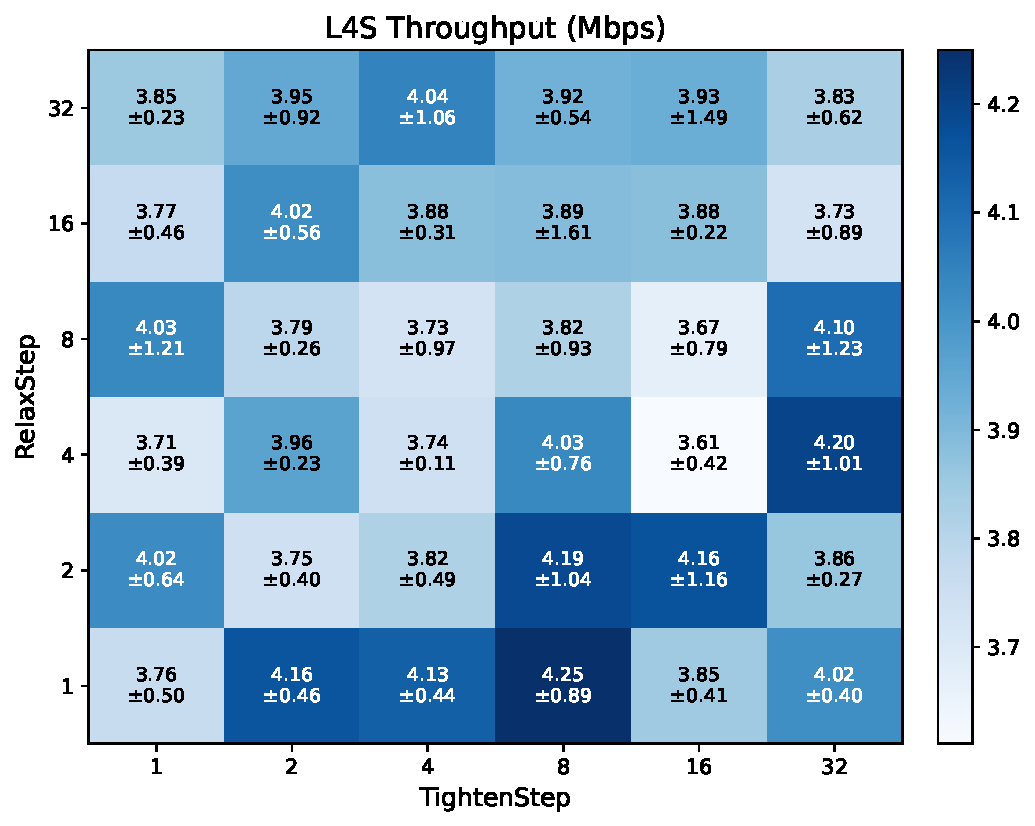
\includegraphics[width=0.88\linewidth]{figures/heatmap_l4s_mbps.pdf}
\caption{L4S throughput across controller step sizes. Dynamic control reduces the dominant L4S share observed in the static configuration. Across the ablation grid, L4S remains in a relatively narrow band around 3.6--4.25 Mbps.}
\label{fig:heatmap-l4s}
\end{figure}

\begin{figure}[t]
\centering
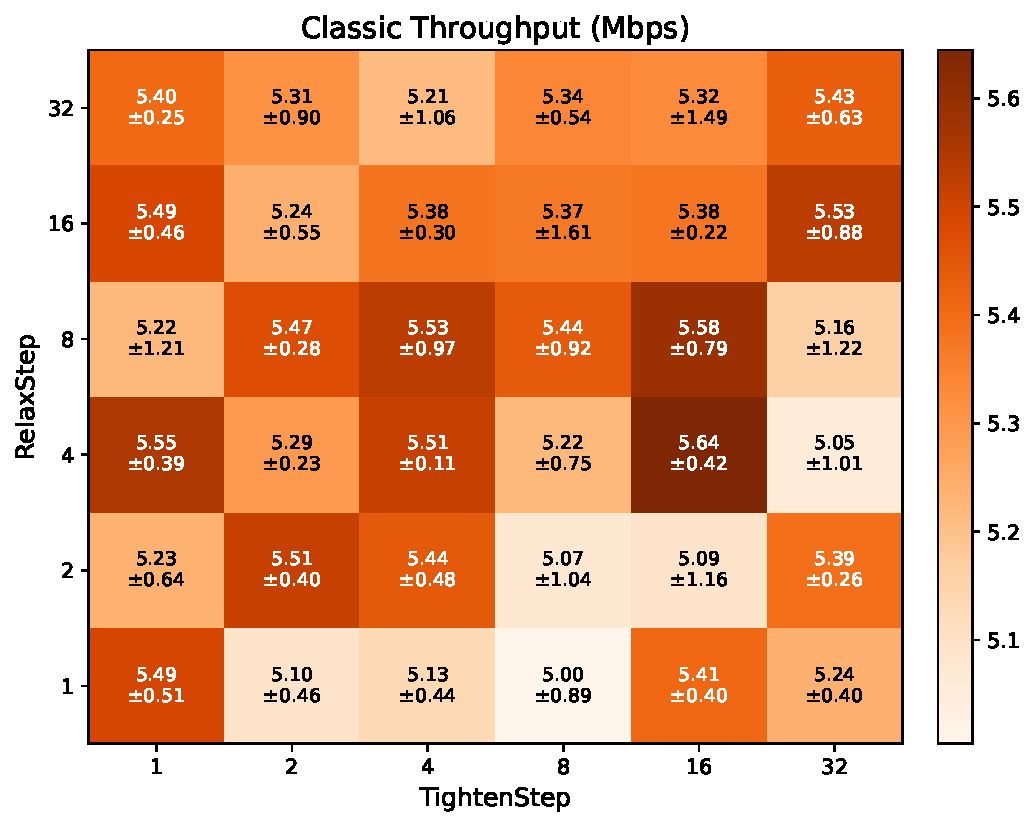
\includegraphics[width=0.88\linewidth]{figures/heatmap_classic_mbps.pdf}
\caption{Classic throughput across controller step sizes. Classic throughput improves from 1.71 Mbps in the static configuration to approximately 5.0--5.64 Mbps in the dynamic configuration.}
\label{fig:heatmap-classic}
\end{figure}

\begin{figure}[t]
\centering
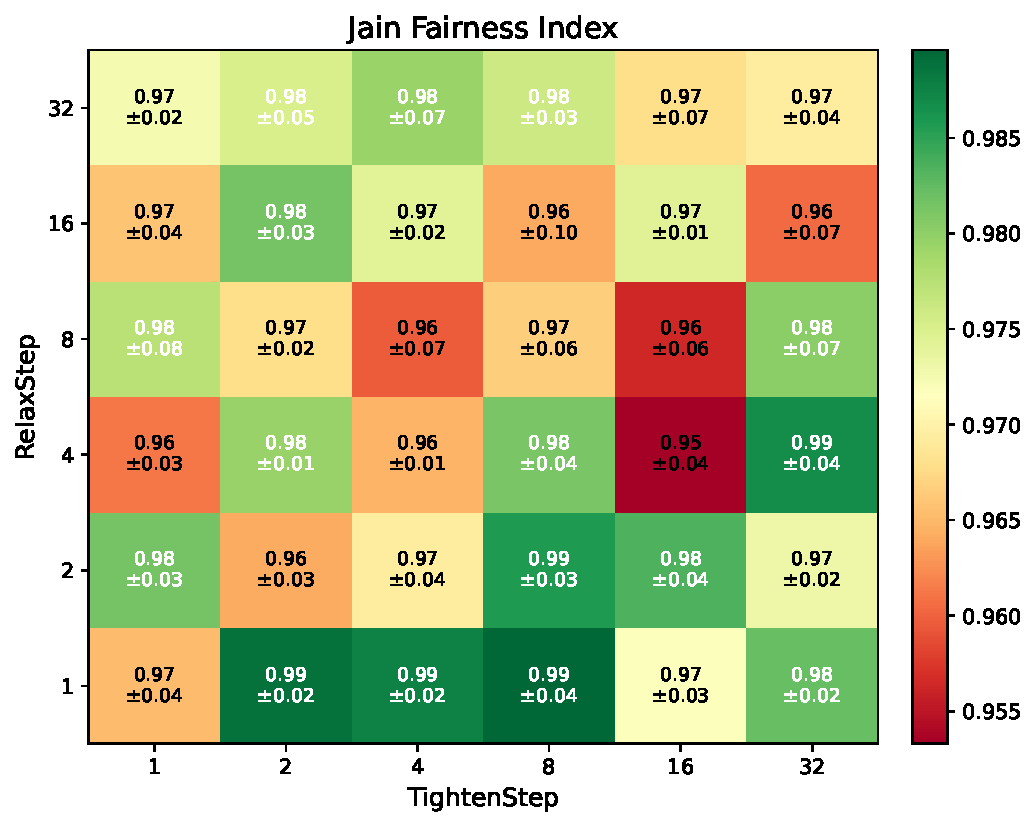
\includegraphics[width=0.88\linewidth]{figures/heatmap_jain_fairness.pdf}
\caption{Jain fairness across controller step sizes. Jain fairness improves from 0.709 in the static configuration to 0.953--0.990 across the dynamic grid. The dynamic settings are therefore much closer to balanced class throughput, although they are slightly Classic-favorable rather than exactly equal.}
\label{fig:heatmap-fairness}
\end{figure}

The highest mean fairness in the sweep occurs at \texttt{relax\_step = 1} and \texttt{tighten\_step = 8}, where L4S obtains 4.25 Mbps, Classic obtains 5.00 Mbps, L4S share is 0.459, and Jain fairness is 0.990. Other high-fairness settings include \texttt{relax\_step = 1} with \texttt{tighten\_step = 2} or \texttt{4}, and \texttt{relax\_step = 2} with \texttt{tighten\_step = 8} or \texttt{16}. These differences should not be over-interpreted because each point has only three trials and several confidence intervals overlap. The robust conclusion is the grid-level shift: dynamic control consistently moves the system from L4S-dominant service toward near-balanced service.

\subsection{Representative confidence-interval plots}

The heatmaps summarize the full ablation grid. Representative error-bar plots for \texttt{relax\_step = 1} show the same trend more directly. The fixed-threshold baseline appears as a horizontal reference line. For L4S throughput, the dynamic values lie well below the fixed reference, confirming that dynamic control reduces L4S dominance. For Classic throughput, the dynamic values lie well above the fixed reference, showing that the lost L4S share is redistributed toward Classic traffic. For Jain fairness, the dynamic values are close to 1, while the fixed reference remains near 0.71.

\begin{figure}[t]
\centering
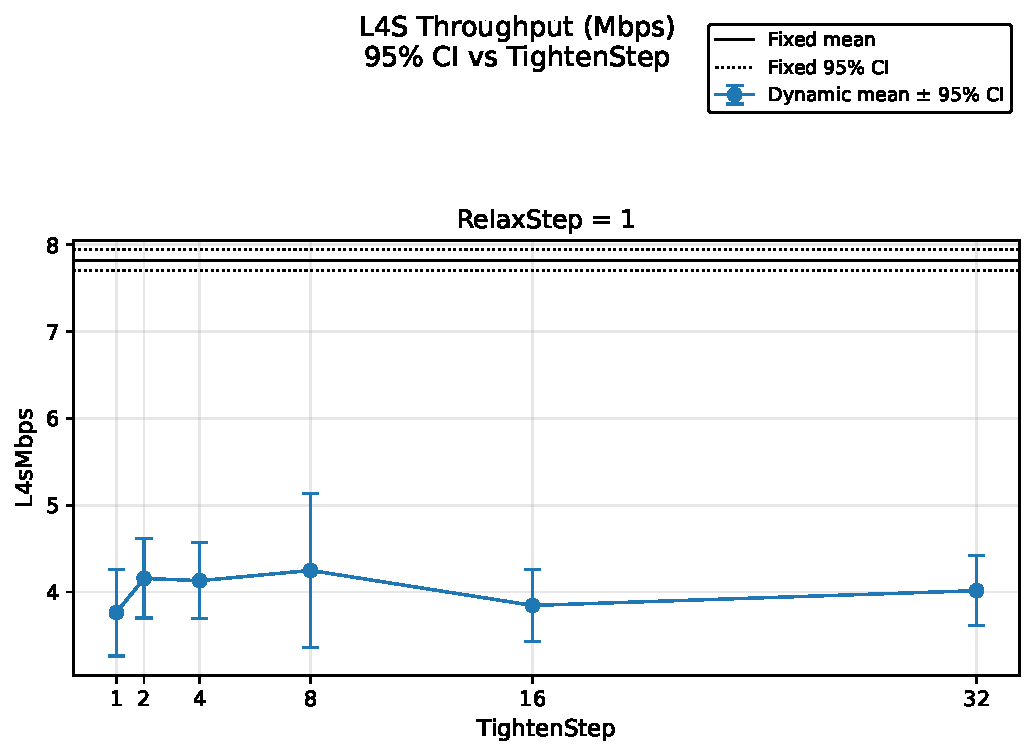
\includegraphics[width=0.86\linewidth]{figures/ci_errorbar_l4s_mbps_relax_1.pdf}
\caption{L4S throughput at \texttt{relax\_step = 1}. Dynamic control lowers the L4S throughput share compared with the static configuration.}
\label{fig:ci-l4s}
\end{figure}

\begin{figure}[t]
\centering
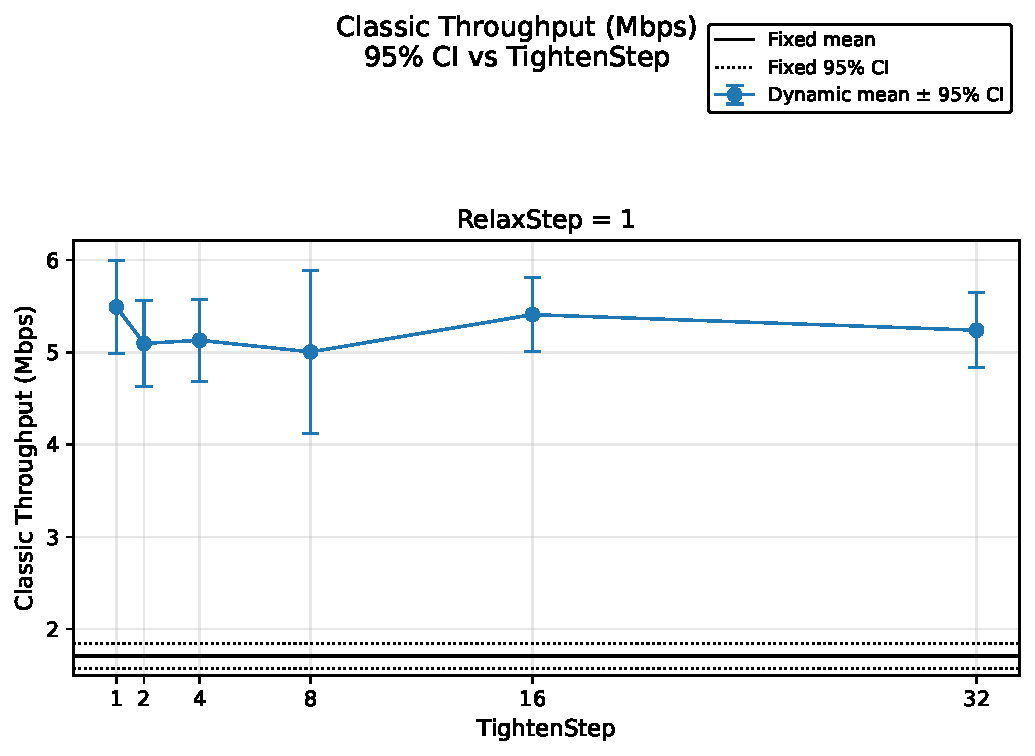
\includegraphics[width=0.86\linewidth]{figures/ci_errorbar_classic_mbps_relax_1.pdf}
\caption{Classic throughput at \texttt{relax\_step = 1}. Classic throughput is consistently higher under dynamic control than under the static configuration.}
\label{fig:ci-classic}
\end{figure}

\begin{figure}[t]
\centering
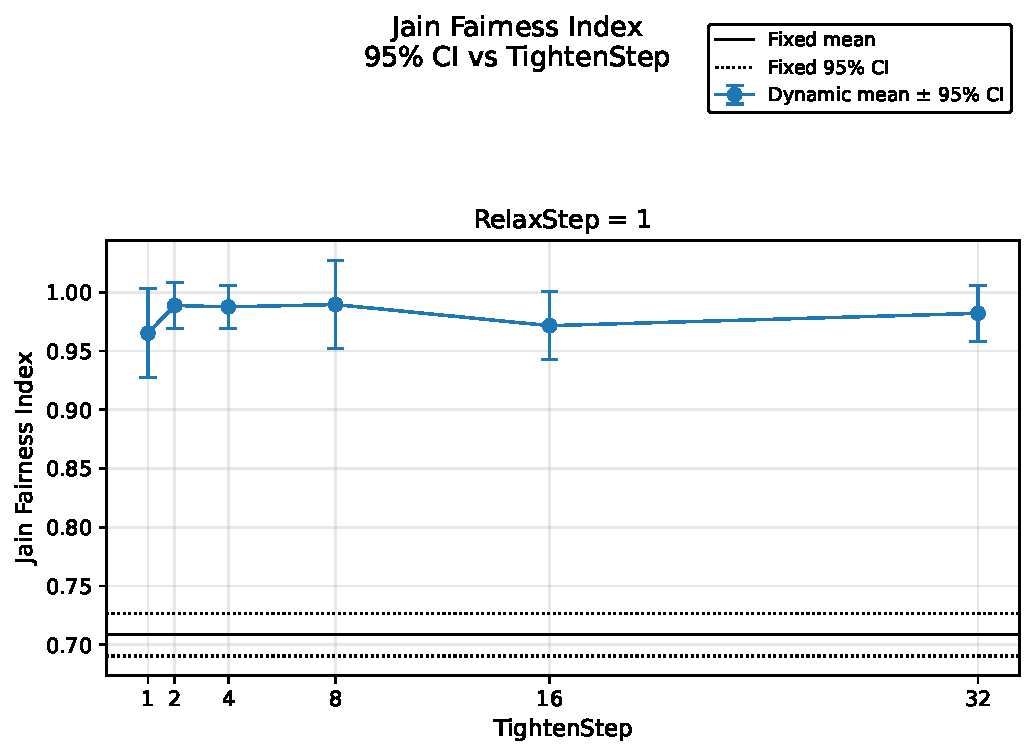
\includegraphics[width=0.86\linewidth]{figures/ci_errorbar_jain_fairness_relax_1.pdf}
\caption{Jain fairness at \texttt{relax\_step = 1}. The dynamic configuration approaches balanced class throughput, while the static configuration remains substantially less fair.}
\label{fig:ci-fairness}
\end{figure}

\subsection{Result interpretation}

The main effect of the controller is redistribution, not additional capacity creation. Because the bottleneck is already overloaded, improving Classic throughput necessarily reduces L4S throughput. This behavior is visible in every dynamic setting: L4S falls from 7.82 Mbps to roughly 4 Mbps, while Classic rises from 1.71 Mbps to roughly 5 Mbps. The dynamic configuration therefore improves coexistence at the cost of weakening the strong L4S preference present in the static configuration.

This is consistent with the implemented mechanism. A lower L4S threshold causes earlier CE marking on L4S packets, and the Classic protection budget can redirect some L4S arrivals into the Classic queue when Classic demand is present. Together, these effects reduce the rate at which the high-priority L4S queue monopolizes the bottleneck. The resulting service split is not an exact implementation of DualQ coupling, but it demonstrates that queue telemetry and controller updates can substantially change class-level fairness in BMv2.

The current results do not establish a complete L4S latency story. The dataplane exports delay-related telemetry and the repository contains packet-capture support, but the final plotted evidence here is throughput and fairness evidence. A full L4S evaluation would additionally report queueing-delay CDFs, p95/p99 delay, CE marking rate, and loss rate for each class across multiple traffic mixes. The present report therefore makes the narrower claim that the dynamic configuration improves Classic coexistence under the tested overload condition.

\section{Discussion}

The implementation shows both the usefulness and the limits of BMv2 for queue-management experiments. BMv2 is expressive enough to support ECN parsing, class-based priority assignment, egress marking, telemetry export, and controller-driven threshold updates. These features are sufficient to build a realistic course-project testbed in which actual TCP traffic crosses a programmable switch. At the same time, BMv2 does not let the P4 program implement a fully custom coupled scheduler. The prototype must therefore be interpreted as an approximation built from available target features.

The Classic protection budget is the most important implementation-specific design choice. Since the P4 ingress pipeline does not have direct access to live Classic queue occupancy, Classic arrivals are used as an approximate signal of Classic demand. This approximation is coarse, but it avoids relying only on dequeue-side Classic telemetry, which can become weak when the Classic queue is receiving little service. The results suggest that the protection mechanism is effective in this workload, because Classic throughput increases by more than 3 Mbps relative to the static configuration.

The controller policy is deliberately simple. It does not estimate an optimal control law, and it does not compute a probabilistic AQM function. Instead, it uses threshold rules based on queue depth, queue growth, and delay signals. This makes the mechanism transparent and easy to ablate. The step-size sweep shows that the broad fairness improvement is not limited to one isolated parameter setting. However, the exact best step size is not a strong scientific result because the confidence intervals overlap and only three trials are used.

One important validity point is that the static and dynamic profiles differ in more than the presence of the controller. The dynamic profile also uses a lower initial L4S threshold, a higher Classic threshold, and a larger Classic protection threshold. The comparison therefore evaluates the static baseline against the complete dynamic fairness configuration, rather than isolating the controller as the only changed variable. This is acceptable for demonstrating the implemented design, but a stricter ablation would separately vary initial thresholds, protection budget, and controller activity.

\section{Limitations and Future Work}

The prototype does not implement standards-faithful DualQ Coupled AQM. It uses BMv2 priority queues and threshold-based CE marking as a practical approximation. A closer implementation would need a target with more programmable traffic-management support, or an external mechanism that can emulate coupled scheduling more directly.

The final evaluation is also narrower than the full motivation of L4S. The project goal includes latency-sensitive service, but the final report figures quantify throughput and fairness rather than queueing-delay distributions. Future evaluation should add latency CDFs and p95/p99 queueing delay for both L4S and Classic traffic. The packet-capture and telemetry infrastructure in the repository provides a starting point for that extension.

The workload is a single-bottleneck, two-class, long-flow experiment with symmetric offered load. Future runs should vary the L4S fraction, offered load, number of flows, RTT, queue depth, burstiness, and controller polling interval. A stronger experimental matrix would include a single FIFO baseline, a static dual-queue baseline without protection, a static dual-queue baseline with protection, and the dynamic design. That matrix would separate the effects of queue separation, static protection, and runtime adaptation.

Finally, the controller uses polling through \texttt{simple\_switch\_CLI}, which is suitable for a BMv2 course project but not for high-rate deployment. A production-oriented design would need a lower-overhead runtime interface and a clearer control-timescale analysis.

\section{Reproducibility Artifact}

The repository contains the P4 program, controller, Mininet topology, traffic generators, evaluation scripts, ablation scripts, tests, and generated report figures. The following commands summarize the main experimental workflow from the repository root. Commands that launch Mininet and BMv2 require root privileges.

\begin{verbatim}
export RUN="sudo env PATH=$PATH PYTHONPATH=."

$RUN python3 topo/topology.py --run-fixed --experiment-duration 180 \
  --l4s-bw 10.0 --classic-bw 10.0 --output-dir results/fixed_run_1

$RUN python3 topo/topology.py --run-fixed --experiment-duration 180 \
  --l4s-bw 10.0 --classic-bw 10.0 --output-dir results/fixed_run_2

$RUN python3 topo/topology.py --run-fixed --experiment-duration 180 \
  --l4s-bw 10.0 --classic-bw 10.0 --output-dir results/fixed_run_3

python3 -m eval.summarize_results results/fixed_run_1
python3 -m eval.summarize_results results/fixed_run_2
python3 -m eval.summarize_results results/fixed_run_3

$RUN python3 scripts/run_ablation.py run
python3 scripts/run_ablation.py analyze
python3 scripts/generate_fixed_baseline_ci.py
python3 scripts/plot_ablation.py
\end{verbatim}

The full dynamic sweep runs 108 experiments and takes several hours on the test machine. The generated \texttt{summary.json}, confidence-interval JSON files, heatmaps, and error-bar plots are sufficient to reproduce the quantitative results reported above.

\section{Conclusion}

This project implemented an L4S-aware queueing prototype in BMv2 using P4, Mininet, a lightweight Python controller, and reproducible evaluation scripts. The dataplane classifies packets by ECN codepoint, separates L4S and Classic traffic into two priority queues, applies threshold-based CE marking in egress, and exports queue telemetry through registers. The control plane adapts thresholds and Classic protection settings at runtime.

The evaluation shows that the static two-queue configuration gives L4S most of the bottleneck capacity, with 7.82 Mbps for L4S, 1.71 Mbps for Classic, and Jain fairness of 0.709. The dynamic fairness configuration shifts the system toward coexistence: across the controller step-size sweep, Classic throughput rises to 5.00--5.64 Mbps and Jain fairness rises to 0.953--0.990, while L4S throughput falls to 3.61--4.25 Mbps. The result is therefore a clear fairness tradeoff. Dynamic threshold control and Classic protection reduce Classic starvation-like behavior, but they do so by reducing L4S dominance.

The completed artifact satisfies the central course-project requirement: it is a working SDN/P4 system with a substantial programming component and a quantitative evaluation. Its main scientific lesson is that L4S-aware class separation is easy to approximate with BMv2 priority queues, but coexistence requires additional protection logic, and the precise latency-fairness behavior depends strongly on the available traffic-manager primitives.

\begin{thebibliography}{9}

\bibitem{rfc9330}
B. Briscoe, K. De Schepper, M. Bagnulo, and G. White,
``Low Latency, Low Loss, and Scalable Throughput (L4S) Internet Service: Architecture,''
RFC 9330, 2023.

\bibitem{rfc9331}
K. De Schepper and B. Briscoe,
``The Explicit Congestion Notification (ECN) Protocol for Low Latency, Low Loss, and Scalable Throughput (L4S),''
RFC 9331, 2023.

\bibitem{rfc9332}
K. De Schepper, B. Briscoe, and G. White,
``Dual-Queue Coupled AQM for Low Latency, Low Loss, and Scalable Throughput,''
RFC 9332, 2023.

\bibitem{p4spec}
P4 Language Consortium,
``P4\_16 Language Specification.''

\bibitem{bmv2}
P4 Behavioral Model,
``BMv2 Simple Switch.''

\bibitem{dctcp}
M. Alizadeh et al.,
``Data Center TCP (DCTCP),''
ACM SIGCOMM, 2010.

\bibitem{pi2p4}
C. Papagianni and K. De Schepper,
``PI2 for P4: An Active Queue Management Scheme for Programmable Data Planes,''
CoNEXT, 2019.

\bibitem{virtualqueues}
H. Harkous et al.,
``Virtual Queues for P4: A Poor Man's Programmable Traffic Manager,''
IEEE Transactions on Network and Service Management, 2021.

\bibitem{l4sscheduler}
S. Nádas et al.,
``A Congestion Control Independent L4S Scheduler,''
Applied Networking Research Workshop, 2020.

\end{thebibliography}

\end{document}
